\documentclass[11pt]{beamer}
\usetheme{default}
\usecolortheme{beaver}
\usepackage[utf8]{inputenc}
\usepackage[english]{babel}
\usepackage{amsmath}
\usepackage{amsfonts}
\usepackage{amssymb}
\author{Corda Francesco - 920212\\
		Damato Davide - 920616\\
		Fiorentino Alessio - 920488\\
		Franchin Luciano - 921093}
\title{Poker Bot}
\subtitle{Project for the Economics and Computation Class\\
		PoliMi 2019-2020}
%\setbeamercovered{transparent} 
%\setbeamertemplate{navigation symbols}{} 
%\logo{} 
%\institute{} 
%\date{} 
%\subject{} 
\begin{document}

\begin{frame}
\titlepage
\end{frame}

%\begin{frame}
%\tableofcontents
%\end{frame}

\begin{frame}{Framework}
\begin{figure}[hbtp]
		\centering
		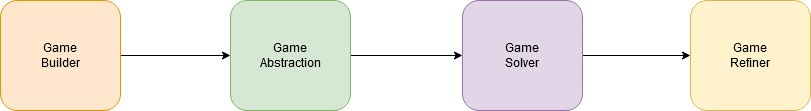
\includegraphics[scale=0.5]{images/img_01.jpg}
		\end{figure}
\end{frame}

\begin{frame}{Game Builder}
\begin{itemize}
\item This module is responsible for the construction of the game tree in extensive form
\item The Game Builder can parse files that comply with the format established by the efg\_lib
\item The parsing is an iterative process that, for each line of the file:
\begin{enumerate}
\item Distinguishes the different classes using a set of regular expressions.
\item Creates a node instance and attach it to the tree.
\item The resulting tree is a recursive data structure of nodes.
\end{enumerate}
\end{itemize}
\end{frame}

\begin{frame}{Game Builder}
\begin{itemize}
\item The game builder also parses the information sets, grouping nodes that belong to the same set together.
\item The information sets are organized in lists of nodes, where each node maintains a reference to the others in the group.
\end{itemize}
\end{frame}

\begin{frame}{Game Abstraction}
\begin{itemize}
\item To perform the game abstraction, we adopted a top-level approach that visits recursively the tree starting from the root. 
\item This choice allowed us to avoid occurrences of imperfect recall during the process.
\item We also designed the algorithm to abstract one player at a time, to be able to use different parameters for each player.
\item Abstraction high level procedure, for each level:
\begin{enumerate}
\item Identifies information sets that are eligible to be unified, based on the sequence of moves that preceded them
\item Produces a clustering
\end{enumerate}
\end{itemize}
\end{frame}

\begin{frame}{Game Abstraction}
\begin{itemize}
\item The clustering task is responsible of grouping information sets that satisfy the following properties:
\begin{itemize}
\item Same player
\item Same level in the tree
\item Same set of actions / sequence of moves that preceded them
\end{itemize}
\item Each node of an information set is associated with a point in a d-dimensional space, where d is the number of terminal nodes that derive from the node. The coordinates in the dimensions are given by the payoffs of the terminal nodes.
\end{itemize}
\end{frame}

\begin{frame}{Game Abstraction}
\begin{itemize}
\item To perform the clustering task, we adopted the K-means algorithm.
\item K-means is one of the most popular clustering algorithm for its simplicity and good performance.
\item As is well known, k-means is not guaranteed to converge to the optimal solution and is strongly dependent on the initialization. To cope with this limitations we tried different random seeds and evaluated the results. 
\item This portion of the project was the only one that we didn't implement, choosing instead to use the implementation provided by the scikit-learn library.
\end{itemize}
\end{frame}

\begin{frame}{Game Solver}
\begin{itemize}
\item After the abstraction, we developed the Game Solver module.
\item This module takes as inputs a game tree and a game abstraction to produce a set strategies for the game.
\item After some research, we decided to adopt a Monte Carlo CFR approach, that guarantees good convergence properties and a faster performances than the standard version of Counterfactual Regret.
\item Also, after some comparisons, we opted for the CFR+ version of the algorithm, because it seemed to provide more stable results.
\end{itemize}
\end{frame}

\begin{frame}{Game Solver}
\begin{itemize}
\item Monte Carlo CFR can be implemented in different ways, depending on the technique used to perform the sampling.
\item We opted for the External Sampling approach, that draws the samples only for the nodes belonging to the opponent and to the nature.
\item Our solution is almost entirely based on the pseudo code developed by Marc Lanctot in his PhD thesis, with the following addition provided by Professor Gatti slides:
\begin{itemize}
\item Each payoff in the terminal nodes is weighted by the inverse of the probability of reaching it, starting from the tree root.
\end{itemize}
\end{itemize}
\end{frame}

\begin{frame}{Game Refiner}
\begin{itemize}
\item The objective of this module is the resolution of an imperfect information game. 
\item Starting from a blueprint strategy produced in the previous step, the Game Refiner improves the strategy at run time by solving an auxiliary tree.
\item To solve the task we adopted again a top down approach, since the optimal strategy at a given level depends on the results from the previous level.
\end{itemize}
\end{frame}

\begin{frame}{Game Refiner}
\begin{itemize}
\item The algorithm traverses the game tree starting from the root. 
\item The main steps for each level are:
\begin{enumerate}
\item Identification of the sub-games in the level.
\item For each sub-game, compression of the sub-tree generated by it. This operation consists in the removal of all the information sets in the sub-tree belonging to the player that we are trying to refine.
\item Creation of an auxiliary tree that associates the sub-games with the probabilities of reaching them from the root node.
\item Solution of the auxiliary tree, using the Game Solver.
\item Remapping of the updated blueprint strategy into the original tree.
\end{enumerate}
\end{itemize}
\end{frame}

\begin{frame}{Performances}
\begin{itemize}
\item To assess the performances of our models, we observed the evolution of the cumulative regret during training.
\item To evaluate the quality of an abstraction, we compare its performance with a baseline (represented by the non-abstracted game).
\item The following plots shows the regret accumulated by an abstraction, compared to a baseline trained with the same parameters.
\end{itemize}
\end{frame}

\begin{frame}{Game Simulator}
\begin{itemize}
\item We built a game simulator to have a closer look at the choices made by the strategies we produced.
\item Given a game tree and a strategy for each player, the Game Simulator plays an arbitrary number of Poker games and outputs:
\begin{itemize}
\item The expected return for each player, computed as the empirical means of the expected rewards collected in each game.
\item The list of moves chosen by the players in each turn, to let us observe the behaviors we were obtaining.
\end{itemize}
\end{itemize}
\end{frame}

\begin{frame}{References}
\begin{itemize}
\item GitHub repository: \url{https://github.com/francescocorda/pokerbot}
\item Slides and videos provided from the Economics and Computation classes
\item Tuomas Sandholm, (2015). Abstraction for solving large incomplete-information games.
\item Marc Lanctot, (2012). Monte Carlo Sampling and Regret Minimization for Equilibrium Computation and Decision-Making in Large Extensive Form Games.

\end{itemize}
\end{frame}

\end{document}